\begin{table}[htpb]
    \centering
    \caption{Some short unfamiliar terminologies in Neural Network}
    {\footnotesize

}
    {\small
    \begin{tabular}{cp{32em}}
        \toprule
        Terminology & Explanations \\
        \midrule
        \makecell{\textbf{i\&o size of conv.} \\ {\color{blue}$[x_w,x_h]\to[x'_w,x'_h]$}} &
        $\begin{array}{rl}
            \left[x_h,~x_w\right] 
            \xrightarrow[\text{pad.}]{[p_h,~p_w]} &
            \left[x_h+2p_h,~x_w+2p_w\right] \\ 
            \xrightarrow[\text{$[s_w,~s_h]$ strided conv.}]{[f_h,~f_w]} &
            \left[\lfloor x_h+2p_h-f_h+1\rfloor,~\lfloor x_w+2p_w-f_w+1\rfloor\right]
        \end{array}$ \\
        \makecell{\textbf{multiple i\&o channels} \\ {\color{blue}$[x_w,x_h,C]\to[x'_w,x'_h,D]$}} &
        $z_{i,j,d}=b_d+\sum_{u=0}^{H-1}\sum_{v=0}^{W-1}\sum_{c=0}^{C-1} x_{\color{red}(si+u),(sj+v),c} w_{u,v,c,d}$, 
        there are a of output channels-number ($D$) of linear weights volumes with size of $[H,W,C]$.   \\
        \makecell{\textbf{pointwise conv.} \\ {\color{blue}$[x_w,x_h,C]\to[x'_w,x'_h,D]$}} &
        $z_{i,j,d}=b_d+\sum_{c=0}^{C-1}x_{i,j,c} w_{0,0,c,d}$, 
        weightedly combining the features across channels at location $(i,j)$ \\
        \makecell{\textbf{dilated conv.}} & 
        $z_{i,j,d}=b_d+\sum_{u=0}^{H-1}\sum_{v=0}^{W-1}\sum_{c=0}^{C-1}x_{\color{red}(i+ru),(j+rv),c}w_{u,v,c,d}$, 
        where $r$ is the dilation factor. 
        It also called \textbf{conv. with holes}, e.g. $\Tilde{\bm{w}}=[w_1,0,w_2,0,w_3]$ if $r=2$ and in 1D conv.,
        resulting in larger receptive field but no more parameters.\\
        
        \makecell{\textbf{pooling} \\ local: {\color{blue}$[x_w,x_h,C]\to[x'_w,x'_h,C]$} \\ or global: {\color{blue}$[x_w,x_h,C]\to[1,1,D]$}} &
        (local) max/average pooling replaces the weighted combinition of normal conv. to $\max(\cdot)$/average and is performed \textit{in each channel independently};
        global max/average pooling \textit{summarize} each channel of feature map into \textit{a single value}. \\
        \textbf{ResNet} & $\bm{x}_{l+1} = \varphi(\bm{x}_l + \mathcal{F}_l(\bm{x}_l))$,
        \textbf{PreResnet} $\bm{x}_{l+1} = \bm{x}_l + \varphi(\mathcal{F}_l(\bm{x}_l))$  \\
        \textbf{DenseNet} & $\bm{x}_{l+1} = \left[\boxed{\bm{x}},\boxed{f_1(\bm{x})}, \boxed{f_2(\bm{x},f_1(\bm{x}))}, \boxed{f_3(\bm{x},f_1(\bm{x}),f_2(\bm{x},f_1(\bm{x})))},\cdots\right]$ \\
        \makecell{\textbf{Auto-ML} \& \textbf{neural} \\
        \textbf{architecture search (NAS)}} & 
        find architectures minimizing the validation loss by derivative-free blackbox optimization methods, 
        which could include multiple objectives, like accuracy, model size, training/inference speed, etc, at the same time. \\
        \makecell{\textbf{depthwise separable conv.} \\ {\color{blue}$[W,H,C]\to[W',H',C]\to[W',H',D]$}} & 
        $z_{i,j,d}=b_d+w'_{c,d}\sum_{c=0}^{C-1}\left(\sum_{u=0}^{H-1}\sum_{v=0}^{W-1}x_{(i+u),(j+u),c}w_{u,v}\right)$. 
        The separable conv. reduces the number of param. from $H\times W\times C\times D$ to $H\times W + C\times D$. \\
        \textbf{activation maximization} & AM, randomize a input pixels of image such that maximize the average activation of a particular neuron 
        to see what the ``neurons'' are learning (simple edges/blobs $\to$ texture patterns $\to$ object parts $\to$ whole objects) \\
        \textbf{DeepDream} & amplify the features from all layers by optimizing the energy function 
        $\mathcal{L}(\bm{x})=\sum_{l\in \mathcal{L}}\Bar{\phi}_l(\bm{x})$,
        where $\Bar{\phi}_l=\frac{1}{HWC}\sum_{h,w,c}\phi_{l,h,w,c}(\bm{x})$ (feature vector for layer $l$). \\
        \textbf{teaching force} & $p(\bm{w}_{1:T}) = \prod_{t=1}^T p(w_t|\bm{w1:t-1})$, conditioned on \textit{ground truth} label. \\
        \textbf{echo state network} & initiate the $\mathbf{W}_\text{h2h}$ with $\lambda\approx 1$ and fix it, then only update $\mathbf{W}_\text{h2o}$. \\
        \textbf{liquid state machine} & constrain the output of a neuron to take value from $\{0,1\}$ \\
        \textbf{reservoir computing} & the generic term of the above two \\
        \bottomrule
    \end{tabular}}
    \label{tab:nn4imgseq}
\end{table}

% The reason why not apply MLP to images:
% \begin{enumerate}[{(1)}]
%     \item The dimension of inputs may be variant, then the size of $\mathbf{W}$ will be different for every image;
%     \item The dimension of inputs, even though fixed, is usually very large, the the size of $\mathbf{W}$ will also be large ($W\times H\times C\times D$) and hard to learn;
%     \item The model may not exhibit \textbf{translation invariance}, since the weights are not shared across locations
% \end{enumerate}


\subsection{Neural Network for Image Data}

The interpretation of the inner production $\bm{w}^\mathsf{T}\bm{x}$: 
comparing the input $\bm{x}$ to a learned template or pattern $\bm{w}$;
the better the match is, the larger the activation is.\unsure{
This interpretation is consistent with the cross-correlation in digital image analysis,
which is to detect local patches (canditate $\bm{x}$) with similar patterns with the target patch (the weight $\bm{w}$).
The candidates, with the same size of target patch, are all possible croppings of the whole image.
} 

\textbf{Convolution} for 2D image, also called \textbf{template matching}, is a form of feature detection, 
and the detected features are called \textbf{feature map} ($\mathbf{Y}$)
\begin{align}
    \mathbf{Y}_{i,j}
    = [\mathbf{W}*\mathbf{X}]_{i,j}
    = \sum_{u=0}^{H-1}\sum_{v=0}^{W-1}w_{u,v}x_{i+u,j+v}
\end{align}

\textbf{Transposed conv.} converts a smaller feature map to a larger one weighted by the kernel.
It comes from the matrix multiplication form of normal conv.:
if $\mathbf{W}$ is derived from the kernel $\mathbf{K}$ by the process in example below,
then 
\begin{gather}
    \mathbf{Y}=\text{transConv}(\mathbf{X},\mathbf{K})\iff\bm{y}=\mathbf{W}^\mathsf{{\color{red}T}}\bm{x}
\end{gather}
It is worth noting that \textbf{Deconv.}, distinct with transposed conv., is the inverse operation of conv., 
which recover the original input with a known filter.



\begin{example}\label{ex:convTconv}
    \textbf{Convolution in matrix multiplication form} \& \textbf{Transposed convolution}
    
    All linear operation can be represented as matrix multiplication form.
    The CNNs can be regarded as a 
    {\begin{align}
        \mathbf{Y}
        =&~ \mathbf{K}*\mathbf{X}~~(\text{from big $\mathbf{X}$ to small $\mathbf{Y}$}) \\
        =&~ \left[\begin{array}{cc}
            {\color{red}k_1}   & {\color{blue}k_2} \\
            {\color{green}k_3} & {\color{violet}k_4}
        \end{array}\right]*\left[\begin{array}{ccc}
            x_1 & x_2 & x_3 \\
            x_4 & x_5 & x_6 \\
            x_7 & x_8 & x_9
        \end{array}\right] \\
        =&~ \left[\begin{array}{cc}
            k_1x_1 + k_2x_2 + k_3x_3 + k_4x_4 & 
            k_1x_2 + k_2x_3 + k_3x_5 + k_4x_6 \\
            k_1x_4 + k_2x_5 + k_3x_7 + k_4x_8 & 
            k_1x_5 + k_2x_6 + k_3x_8 + k_4x_9
        \end{array}\right] \\
        \iff \notag\\
        \bm{y} 
        =&~ \mathbf{W}\bm{x} \\
        =&~ \left[\begin{array}{ccc|ccc|ccc}
            {\color{red}k_1}     & {\color{blue}k_2}   & 0                   & 
            {\color{green}k_3}   & {\color{violet}k_4} & 0                   & 
            0                    & 0                   & 0                   \\
            0                    & {\color{red}k_1}    & {\color{blue}k_2}   & 
            0                    & {\color{green}k_3}  & {\color{violet}k_4} & 
            0                    & 0                   & 0                   \\
            0                    & 0                   & 0                   & 
            {\color{red}k_1}     & {\color{blue}k_2}   & 0                   & 
            {\color{green}k_3}   & {\color{violet}k_4} & 0                   \\
            0                    & 0                   & 0                   & 
            0                    & {\color{red}k_1}    & {\color{blue}k_2}   & 
            0                    & {\color{green}k_3}  & {\color{violet}k_4} \\
        \end{array}\right]\left[\begin{array}{c}
            x_1 \\ x_2 \\ x_3 \\ x_4 \\ x_5 \\ x_6 \\ x_7 \\ x_8 \\ x_9
        \end{array}\right] \\
        =&~ \left[\begin{array}{c}
            k_1x_1 + k_2x_2 + k_3x_3 + k_4x_4 \\ k_1x_2 + k_2x_3 + k_3x_5 + k_4x_6 \\
            k_1x_4 + k_2x_5 + k_3x_7 + k_4x_8 \\ k_1x_5 + k_2x_6 + k_3x_8 + k_4x_9
        \end{array}\right]
    \end{align}}
    The transposed CNNs can be regarded as 
    \begin{align}
        \mathbf{Y}
        =&~ \mathbf{K}**\mathbf{X}~~(\text{small $\mathbf{X}$ to big $\mathbf{Y}$}) \\
        =&~ \left[\begin{array}{cc}
            {\color{red}k_1}   & {\color{blue}k_2} \\
            {\color{green}k_3} & {\color{violet}k_4}
        \end{array}\right]**\left[\begin{array}{cc}
            x_1 & x_2 \\
            x_3 & x_4 
        \end{array}\right] \\
        =&~ \left[\begin{array}{ccc}
            {\color{red}k_1}x_1                                                                         & 
            {\color{red}k_1}x_2 + {\color{blue}k_2}x_1                                                  & 
            {\color{blue}k_2}x_2                                                                        \\
            {\color{red}k_1}x_3 + {\color{green}k_3}x_1                                                 & 
            {\color{red}k_1}x_4 + {\color{blue}k_2}x_3 + {\color{green}k_3}x_2 + {\color{violet}k_4}x_1 & 
            {\color{blue}k_2}x_4 + {\color{violet}k_4}x_2                                               \\
            {\color{green}k_3}x_3                                                                       & 
            {\color{green}k_3}x_4 + {\color{violet}k_4}x_3                                              & 
            {\color{violet}k_4}x_4                                                                      \\
        \end{array}\right] \\
        \iff \notag\\
        \bm{y} 
        =&~ \mathbf{W}^\mathsf{T}\bm{x} \\
        =&~ \left[\begin{array}{cccc}
            {\color{red}k_1}     & 0                   & 0                   & 0                    \\
            {\color{blue}k_2}    & {\color{red}k_1}    & 0                   & 0                    \\
            0                    & {\color{blue}k_2}   & 0                   & 0                    \\
            {\color{green}k_3}   & 0                   & {\color{red}k_1}    & 0                    \\
            {\color{violet}k_4}  & {\color{green}k_3}  & {\color{blue}k_2}   & {\color{red}k_1}     \\
            0                    & {\color{violet}k_4} & 0                   & {\color{blue}k_2}    \\
            0                    & 0                   & {\color{green}k_3}  & 0                    \\
            0                    & 0                   & {\color{violet}k_4} & {\color{green}k_3}   \\
            0                    & 0                   & 0                   & {\color{violet}k_4}  
        \end{array}\right]\left[\begin{array}{c}
            x_1 \\ x_2 \\ x_3 \\ x_4
        \end{array}\right] 
        = \left[\begin{array}{c}
            {\color{red}k_1}x_1 \\
            {\color{blue}k_2}x_1 + {\color{red}k_1}x_2 \\
            {\color{blue}k_2}x_2 \\
            {\color{green}k_3}x_1 + {\color{red}k_1}x_3 \\
            {\color{violet}k_4}x_1 + {\color{green}k_3}x_2 + {\color{blue}k_2}x_3 + {\color{red}k_1}x_4 \\
            {\color{violet}k_4}x_2 + {\color{blue}k_2}x_4 \\
            {\color{green}k_3}x_3 \\
            {\color{violet}k_4}x_3 + {\color{green}k_3}x_4 \\
            {\color{violet}k_4}x_4
        \end{array}\right]
    \end{align}
    
\end{example}

\begin{table}[htpb]
    \centering
    {\small
    \begin{tabular}{cp{26em}p{8em}}
        \toprule
        tasks & outputs & models \\
        \midrule
        \textbf{image tagging}          & $\mathcal{Y}=\{0,1\}^C$                           & - \\
        \textbf{objective detection}    & a set of bounding boxes with their class labels' probabilities:
        $\bm{f}_{\bm{\theta}}: \mathbb{R}^{H\times W\times K}\to[0,1]^{A\times A}\times\{1,\cdots,C\}^{A\times A}\times \left(A^4\right)^{A\times A}$,
        where $A\times A$ represent the coord. for $A$ \textbf{anchor boxes} & singleshot detector, YOLO \\
        \textbf{instance segmentation}  & 2D shape mask of each object instance in the image with its label & Mask R-CNN \\
        \textbf{semantic segmentation}  & a class label $y_i\in\{1,\cdots,C\}$ for each pixel. The labels could be depth, surface orientation, etc. & U-Net (enc-dec) \\
        \textbf{human pose estimation}  & the locations of a fixed set of skeletal keypoints  & PersonLab, OpenPose \\
        \bottomrule
    \end{tabular}}
    \caption{Other discriminative vision tasks with CNNs}
    \label{tab:vistasks}
\end{table}

\textbf{Normalization layers}: 
\textit{standardize} the statistics of hidden units to remit the problems of \textit{vanishing or exploding gradients}.
\textbf{Batch normalization (BN)}
(i) makes the optimization landscape significant smoother, 
(ii) reduces the sensitivity to the learning rate, and 
(iii) acts like a regularizer and equivalent to a form of approximate Bayesian inference.
\begin{gather}
    \Tilde{\bm{z}}_n=\mathrm{BN}(\bm{z}_n;\bm{\theta})=\bm{\gamma}\odot\hat{\bm{z}}_n+\bm{\beta},~
    \text{where}~\hat{\bm{z}}_n=\frac{\bm{z}_n-\bm{\mu}_\mathcal{B}}{\sqrt{\bm{\sigma}_\mathcal{B}^2+\epsilon}}
\end{gather}
where $\bm{\mu}_\mathcal{B}$ and $\bm{\sigma}_\mathcal{B}^2$ have the same dimension with channels (treat channel independently).
It should be noted that, besides the \uline{learned parameter $\bm{\gamma}$ and $\bm{\beta}$}, 
the whole training set's $\bm{\mu}_{\mathcal{B}_\text{tr}}$ and $\bm{\sigma}_{\mathcal{B}_\text{tr}}^2$ 
are also kept as parameters to standardize the testing sample(s).
When it is combined with a linear layer, called \textbf{fused batchnorm}, the speed can boost:
\begin{gather}
    \bm{\gamma}\odot(\mathbf{XW}+\bm{b}-\bm{\mu})/\bm{\sigma}+\bm{\beta} \iff \mathbf{XW}'+\bm{b}'
\end{gather}
where $\mathbf{W}'=\bm{\gamma}\odot\mathbf{W}/\bm{\sigma}$ and $\bm{b}'=\bm{\gamma}\odot(\bm{b}-\bm{\mu})/\bm{\sigma}+\bm{\beta}$.

\begin{figure}[htpb]
    \centering
    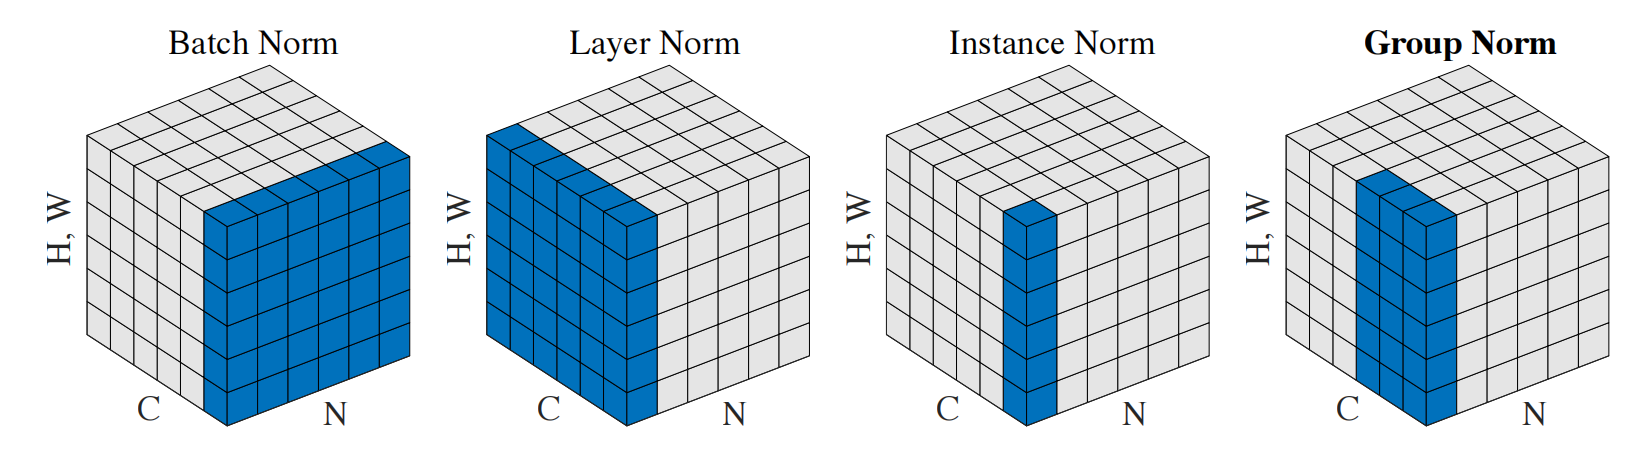
\includegraphics[width=0.8\textwidth]{figs/cnnnormlayer.png}
    \caption{Normalization methods for a CNN}
    {\footnotesize
    \textbf{BN}: pool over height and width in a batch, but match on the channel;
    \textbf{LN}: pool over channel, height and width, but match on the instance index in a batch;
    \textbf{IN}: pool over each instance in the batch and for each channel;
    \textbf{GN}: pool over all locations whose channel is in the same group.
    }
    \label{fig:cnnnormlayer}
\end{figure}

\textbf{Metropolis-adjusted Langevin algorithm (MALA)}: 
sample (generate) images from a generative image model based on trained classifier 
(on current image data), $p(y=c|\bm{x})$, and specified image prior, $p(\bm{x})$,
and under the assumption of normal error\unsure{
{\color{red} This part in \textit{PML: Intro} is in lack of details}
}:
\begin{align}
    p(\bm{x}|y)                     \propto&~     p(\bm{x})p(y|\bm{x}) \\
    \mathcal{E}_c(\bm{x})           \triangleq&~  \log\underbrace{p(y=c|\bm{x})}_\text{trained clf} + \log{\color{teal}p(\bm{x})}~\text{\color{teal}image prior} \\
    \bm{x}'                         =&~           \bm{x} + \frac{\epsilon}{2}\nabla\log{\mathcal{E}_c(\bm{x})} + \mathcal{N}(\mathbf{0},\epsilon\mathbf{I}),~\text{or} \\
    \bm{x}_{t+1}                    =&~           \bm{x}_t 
        + \underbrace{\epsilon_1\nabla_{\bm{x}}\log{p(\bm{x}_t)}}_{\text{plausible under pror}} 
        + \underbrace{\epsilon_2\nabla_{\bm{x}}\log{p(y=c|\bm{x}_t)}}_{\text{plausible under likelihood}} 
        + \underbrace{\mathcal{N}(\mathbf{0},\epsilon_3^2\mathbf{I})}_{\text{intro. randomness}} \label{eq:mala3eps}
\end{align}
\begin{itemize}
    \item \textbf{Gaussian prior}: $p(\bm{x})=\mathcal{N}(\bm{x}|\mathbf{0},\mathbf{I})$, 
    then $\nabla_{\bm{x}}\log{p(\bm{x}_t)}=-\bm{x}_t$ in Equation (\ref{eq:mala3eps});
    \item \textbf{Total variation (TV) prior}: $p(\bm{x})\propto\exp{(-\mathrm{TV}(\bm{x}))}$, 
    where $\mathrm{TV}(\bm{x})$ is \textbf{TV norm}
    \begin{gather}
        \mathrm{TV}(\bm{x})=\sum_{i,j,k}[
            (\underbrace{x_{i,j,k}-x_{(i+1),j,k}}_\text{horizontal Sobel})^2 + 
            (\underbrace{x_{i,j,k}-x_{i,(j+1),k}}_\text{vertical Sobel})^2
        ]
    \end{gather}
\end{itemize}

\textbf{Neural style transfer}: 
generate a new image $\bm{x}$ that re-renders $\bm{x}_c$ in the style of $\bm{x}_s$ 
by optimizing the following energy function
\begin{gather}
    \mathcal{L}(\bm{x}|\bm{x}_s,\bm{x}_c) 
    = \lambda_{\mathrm{TV}}\mathcal{L}_{\mathrm{TV}}(\bm{x}) 
    + \lambda_c\mathcal{L}_{\text{content}}(\bm{x},\bm{x}_c)
    + \lambda_s\mathcal{L}_{\text{style}}(\bm{x},\bm{x}_s) 
\end{gather}
where 
\begin{itemize}
    \item $\mathcal{L}_{\text{content}}$ describes the content similarity between $\bm{x}$ and $\bm{x}_c$ 
    by comparing feature maps of a pre-trained CNN $\phi(\bm{x})$ in the relevant ``content layer'' $l$;
    \begin{gather}
        \mathcal{L}_{\text{content}}(\bm{x},\bm{x}_c)=\frac{1}{C_lH_lW_l}\|\phi_l(\bm{x})-\phi_l(\bm{x}_c)\|_2^2
    \end{gather}
    \item $\mathcal{L}_{\text{style}}$ describes the style similarity between $\bm{x}$ and $\bm{x}_c$
    by interpret visual style as the statistical distribution of certain features that are free from location.
    \begin{align}
        \mathcal{L}_{\text{style}}(\bm{x},\bm{x}_s) =&~
        \sum_{l\in\mathcal{S}}\mathcal{L}_\text{style}^l(\bm{x},\bm{x}_s) \\
        \mathcal{L}_\text{style}^l(\bm{x},\bm{x}_s) =&~
        \|\mathbf{G}_l(\bm{x})-\mathbf{G}_l(\bm{x}_s)\|_F^2 \\
        G_l(\bm{x})_{c,d} =&~ 
        \frac{1}{H_lW_l}\sum_{h=1}^{H_l}\sum_{w=1}^{W_l}\phi_l(\bm{x})_{h,w,c}\phi_l(\bm{x})_{h,w,d}
    \end{align}
\end{itemize}


\subsection{Neural Network for Sequence Data}

\textbf{Forms of RNNs}: transform among embeddings and sequences\unsure{where a initial state $\bm{h}_0$ is assigned in advance.}
\begin{itemize}
    \item sequence generation (\textbf{Vec2Seq}): $f_{\bm{\theta}}:\mathbb{R}^D\to\mathbb{R}^{N_\infty C}$ (from vec $\bm{x}$ to seq $\bm{y}_{1:T}$)
    \begin{align}
        p(\bm{y}_{1:T}|\bm{x}) &=~ \sum_{h_{1:T}}\prod_{t=1}^Tp(\bm{y}_t|\bm{h}_t)p(\bm{h}_t|\bm{h}_{t-1},\bm{y}_{t-1},\bm{x}) \\
        p(\bm{y}_t|\bm{h}_t) &=~ \underbrace{\begin{cases}
        \mathrm{Cat}(\bm{y}_t|\mathrm{softmax}(\mathbf{W}_\text{h2y}\bm{h}_t+\bm{b}_\text{h2y})) ~\text{or}\\
        \mathcal{N}(\bm{y}_t|\mathbf{W}_\text{h2y}\bm{h}_t+\bm{b}_\text{h2y},\sigma^2\mathbf{I})
        \end{cases}}_\text{the only stochasticity}\\
        p(\bm{h}_t|\bm{h}_{t-1},\bm{y}_{t-1},\bm{x}) &=~ \underbrace{\mathbb{I}(\bm{h}_t = f(\bm{h}_{t-1},\bm{y}_{t-1},\bm{x}))}_\text{deterministically computed} \\
        f(\bm{h}_{t-1},\bm{y}_{t-1},\bm{x}) &=~ \varphi(\mathbf{W}_\text{x2h}[\bm{x};\bm{y}_{t-1}]+\mathbf{W}_\text{h2h}\bm{h}_{t-1}+\bm{b}_\text{h}) \label{eq:vec2seqh}
    \end{align}

    \item sequence classification (\textbf{Seq2Vec}): $f_{\bm{\theta}}:\mathbb{R}^{TD}\to\mathbb{R}^{C}$ (from seq $\bm{x}_{1:T}$ to vec $\bm{y}$)
    \begin{align}
        p(y|\bm{x}_{1:T}) 
        =&~ \mathrm{Cat}(y|\mathrm{softmax}(\mathbf{W}\bm{h}^*)) \\
        \bm{h}^*
        =&~ \begin{cases}
            \bm{h}^\rightarrow_T & \text{unidirectional, or} \\
            \Bar{\bm{h}} = \frac{1}{T}\sum_{t=1}^T[\bm{h}^\rightarrow_t,\bm{h}^\leftarrow_t] & \text{bidirectional},~\text{where}
        \end{cases}\\
        % \text{where}~\bm{h}_t 
        % = \varphi(\mathbf{W}_\text{x2h}\bm{x}_{t-1}+\mathbf{W}_\text{h2h}\bm{h}_{t-1}+\bm{b}_\text{h}),\\
        \bm{h}^\rightarrow_t =&~ \varphi(\mathbf{W}^\rightarrow_\text{x2h}\bm{x}_t + \mathbf{W}^\rightarrow_\text{h2h}\bm{h}^\rightarrow_{\color{green}t-1} + \bm{b}^\rightarrow_\text{h}) \label{eq:seq2vech1} \\
        \bm{h}^\leftarrow_t =&~ \varphi(\mathbf{W}^\leftarrow_\text{x2h}\bm{x}_t + \mathbf{W}^\leftarrow_\text{h2h}\bm{h}^\leftarrow_{\color{red}t+1} + \bm{b}^\leftarrow_\text{h}) \label{eq:seq2vech2}
    \end{align}
    
    \item sequence translation (\textbf{Seq2Seq}): $f_{\bm{\theta}}:\mathbb{R}^{TD}\to\mathbb{R}^{T'D}$ (from seq $\bm{x}_{1:T}$ to $\bm{y}_{1:T'}$)\unsure{which can be regarded as labeling every token in a sequence}.
    \begin{align}
        p(\bm{y}_{1:T}|\bm{x}_{1:T'})=&~\begin{cases}
            \sum_{\bm{h}_{1:T}}\prod_{t=1}^T p(\bm{y}_t|\bm{h}_t^L)\mathbb{I}(\bm{h}_t^L 
            = f_L(\bm{h}_{t-1}^L,\bm{x}_t)) & T=T' \\
            f_d(\bm{c})~\text{and}~\bm{c}
            = f_e(\bm{x}_{1:T}) & T \neq T'
        \end{cases} \\
        f_l(\bm{h}_{t-1}^l,\bm{x}_t)
        =&~ \varphi_l(\mathbf{W}_\text{x2h}^l\bm{h}_t^{l-1} + \mathbf{W}_\text{h2h}^l\bm{h}_{t-1}^l + \bm{b}_\text{h}^l) \label{eq:seq2seqh} \\
        p(\bm{y}_t|\bm{h}_t^L)
        =&~ \mathrm{Dist}(\bm{y}_t|\bm{o}_t = \mathbf{W}_\text{h2o}\bm{h}_t^L + \bm{b}_\text{o})
    \end{align}
    where $\bm{c}$ is the context vector encoding the information of input sequence, 
    forming a bottle neck of \textbf{enc-dec architecture}.
\end{itemize}

\textbf{Backpropagation through time}: For the flattened version ${\color{teal}\bm{w}_\text{h}}$ of $[{\color{teal}\mathbf{W}_\text{h2h},\mathbf{W}_\text{h2w}}]$,\unsure{
the expansion is due to the {\color{teal}shared parameters $\bm{w}_\text{h}$ for all $t=0,1,\cdots,T$}
and the {\color{purple}hidden states $\bm{h}_\cdot$, acting as output at current time and input at next time for the same function $f$}.
}
\begin{align}
    \mathcal{L} =&~ \frac{1}{T}\ell{(y_t,\bm{o}_t)} \\
    {\color{purple}\bm{h}_t} =&~ f(\bm{x}_t,{\color{purple}\bm{h}_{t-1}},{\color{teal}\bm{w}_\text{h}}) \\
    \bm{o}_t =&~ g(\bm{h}_t,\bm{w}_\text{o}) \\
    \frac{\partial\mathcal{L}}{\partial{\color{teal}\bm{w}_\text{h}}} 
    =&~ \frac{1}{T}\sum_{t=1}^T
        \frac{\partial\ell(y_t,\bm{o}_t)}{\partial\bm{o}_t}
        \frac{\partial g(\bm{h}_t,\bm{w}_\text{o})}{\partial\bm{h}_t}
        \frac{\partial\bm{h}_t}{\partial{\color{teal}\bm{w}_\text{h}}} \\
    \frac{\partial\bm{h}_t}{\partial{\color{teal}\bm{w}_\text{h}}}
    =&~ \frac{\partial f(\bm{x}_t,\bm{h}_{t-1},{\color{teal}\bm{w}_\text{h}})}{\partial{\color{teal}\bm{w}_\text{h}}}\\
        &+ \sum_{i=1}^{t-1}
        \underbrace{\left(
            \prod_{j=i+1}^t\frac{\partial f(\bm{x}_j,\bm{h}_{j-1},{\color{teal}\bm{w}_\text{h}})}{\partial\bm{h}_{j-1}}
        \right)}_\text{\makecell{causing vanishing or \\exploding gradient problems}}
        \frac{\partial f(\bm{x}_j,\bm{h}_{i-1},{\color{teal}\bm{w}_\text{h}})}{\partial{\color{teal}\bm{w}_\text{h}}}
\end{align}
which requires $O(T^2)$ time to compute for a entire sequence. 
This problem can be handled by truncating the original long sequence into several subsequences lengthing $K$.\unsure{
which requires $O(TK)$ time. The gradients also propagate within the $K$ steps, may causing a $K$-gram model.
}
The update should be relayed across ordered subsequences but reset across random ones.

\begin{figure}[htpb]
    \centering
    \begin{subfigure}[t]{0.45\textwidth}
    \centering
    \label{fig:gru}
    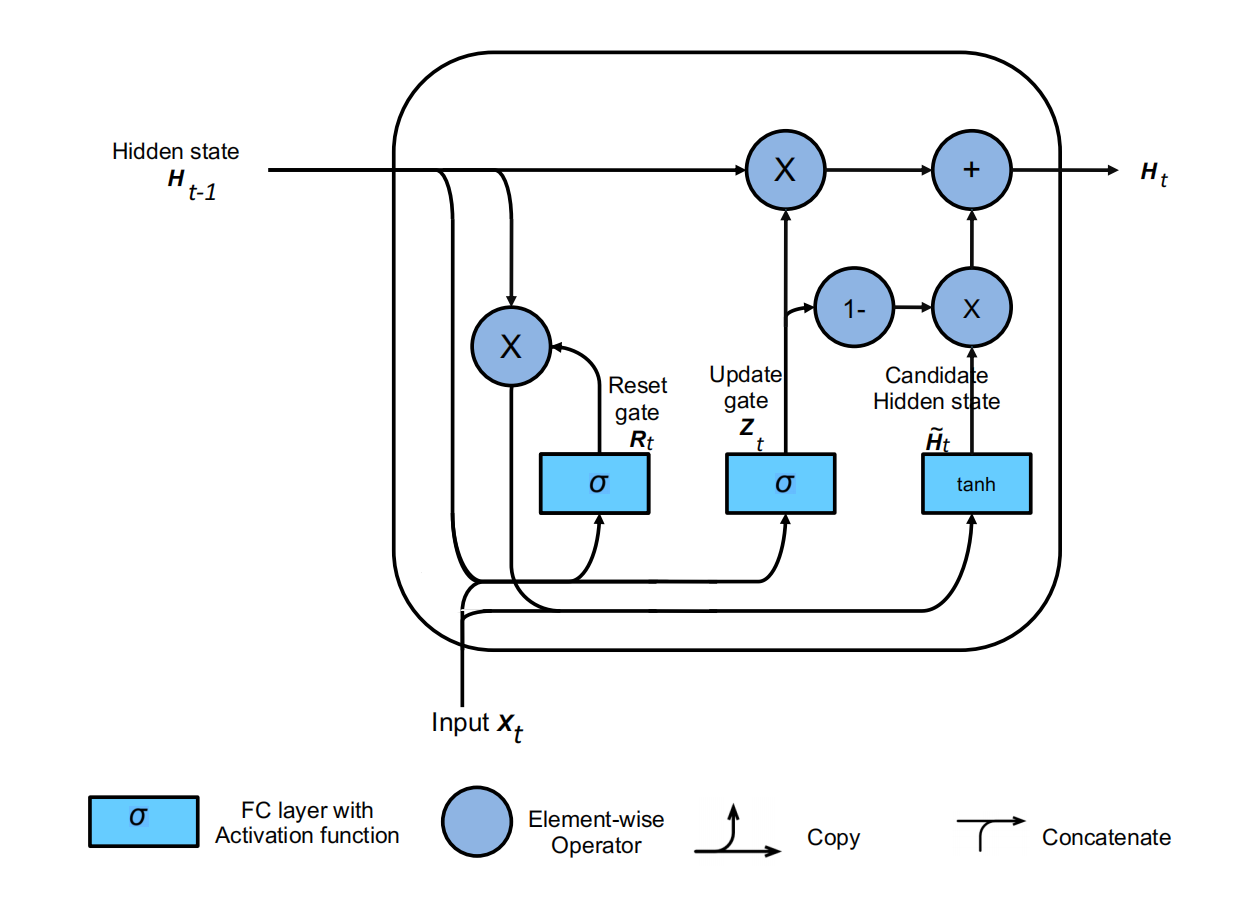
\includegraphics[width=\textwidth]{figs/gru.png}
    \caption{GRU (Gated recurrent units)}
    {\footnotesize
    $\mathbf{H}_t
    = \mathbf{Z}_t\odot\mathbf{H}_{t-1}
    + (1-\mathbf{Z}_t)\odot\Tilde{\mathbf{H}}_t$
    }
    \end{subfigure}
    \begin{subfigure}[t]{0.45\textwidth}
    \centering
    \label{fig:lstm}
    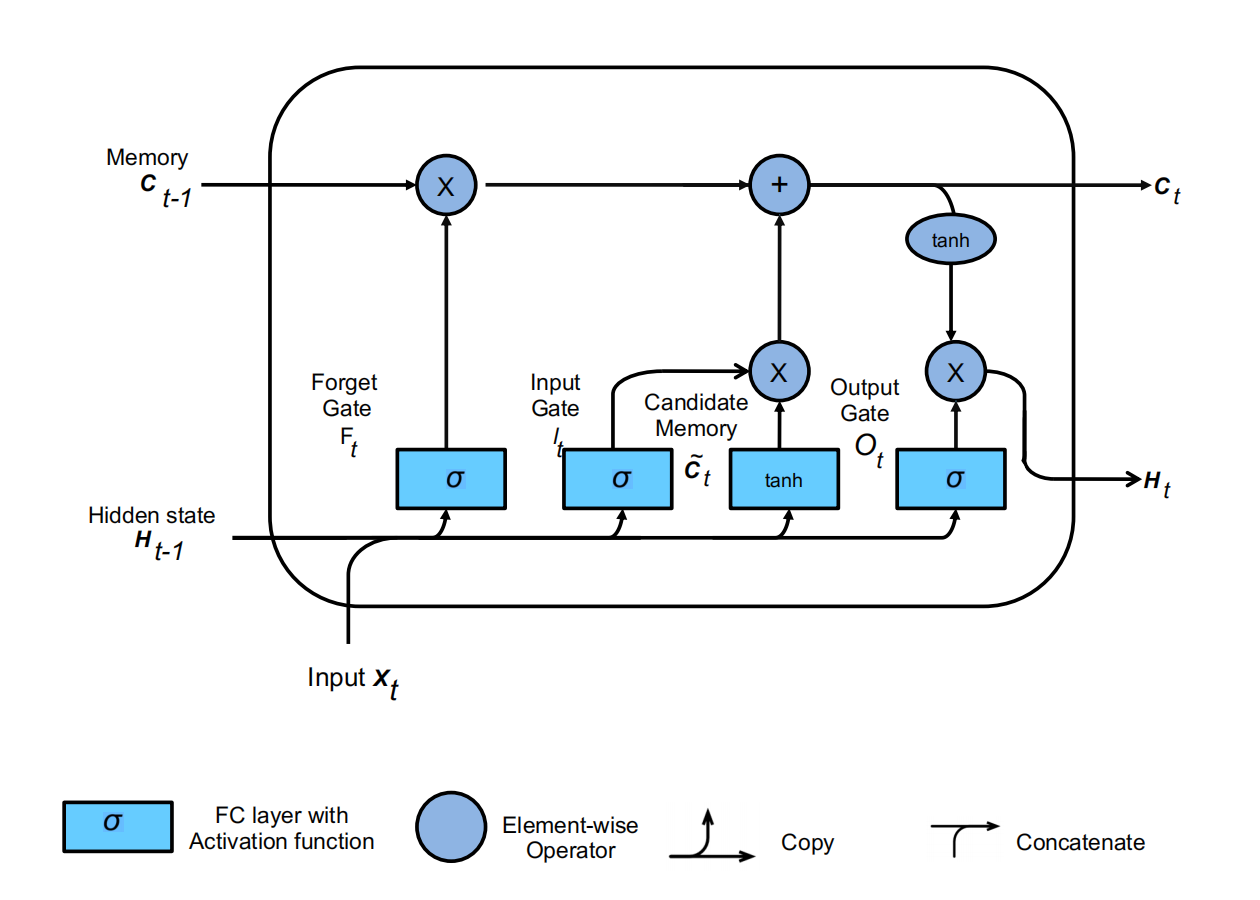
\includegraphics[width=\textwidth]{figs/lstm.png}
    \caption{LSTM (Long short term memory)}
    {\footnotesize
    $\mathbf{C}_t=\mathbf{F}_t\odot\mathbf{C}_{t-1}+\mathbf{I}_t\odot\Tilde{\mathbf{C}}_t$\\
    $\mathbf{H}_t=\mathbf{O}_t\odot\mathrm{tanh}(\mathbf{C}_t)$
    }
    \end{subfigure}
    \caption{Gating and long term momory}
    {\footnotesize
    Since gradient vanishing, the vanilla RNNs fail to remember inputs from long in the past.
    The problem is solved by specify the update of hidden state.
    }
    \label{fig:grulstm}
\end{figure}





\textbf{Beam search}: a heuristic method for decoding a sequence 
by trying top $K$ possible words in each step and record these paths and their probabilities, similar with \textbf{Viterbi algorithm} in decoding a hidden Markov chain.\unsure{
If $K=1$, it gets back to greedy searching that only records the highest possible word in each step, which only achieve a local minimum; 
or if $K=V$, it tries all possibilities and reaches the global optimum but will have $O(V^T)$ complexity of time.
}

\textbf{Causal CNN}, also called \textbf{convolutional Markov model},
is a generative model\unsure{
Recall the generative classifier in Chapter 9, which regards the output $\bm{y}$ is the model's parameters.
}
based on 1D CNN for sequence data but masked out future inputs,
where each output variable, including hidden states, only depends on \textit{previously} generated variables
\begin{gather}
    p(\bm{y})
    = \prod_{t=1}^T p(y_t|\bm{y}_{1:t-1})
    = \prod_{t=1}^T \mathrm{Cat}(y_t|\mathrm{softmax}(\varphi(\sum_{\tau=1}^{t-k}\bm{w}^\mathsf{T}\bm{y}_{\tau:\tau+k}))).
\end{gather}
The long-range dependencies and high-level relationship can be achieved by deeper model (current output, hidden states, as inputs of the next layer) and dilated convolution, both can extend the receptive field of conv. operations, such as the text2speech synthesis system, \textit{wavenet}.
